%Packages
\documentclass[12pt]{article}
 \usepackage{times}
\usepackage{fullpage}
\usepackage{setspace}
\usepackage{graphicx}

\begin{document}
\pagestyle{empty}

%\raggedright
\noindent {\bf Meta-analysis of the development of disambiguation behavior}\\
{\bf Poster} (word count = 532) 

 \vspace{5mm}
 
\noindent Faced with a novel word, children have a robust bias to assume that word refers to a novel object, as opposed to an object for which the child already knows the name (e.g., Markman \& Wachtel, 1988;  E. Clark, 1987, 1988). This disambiguation (or ``mutual exclusivity'')  bias has  been suggested as an important means by which children learn new words. However, despite its potential importance in word learning, the underlying cognitive supports of this behavior are unknown. This is because there are a number of theoretical alternatives that could explain disambiguation behavior and they are difficult to disentangle empirically. For example, children could rely on an in-the-moment pragmatic judgement about the speakers intention, or more-general knowledge that the lexicon is structured to have a one-to-one mapping between words and concepts, or both. Each alternative makes nearly identical empirical predictions in any individual experiment, and studies that have attempted to  disentangle them more directly have yielded conflicting results (e.g., Diesendruck \& Markson, 2001; Preissler \& Carey, 2005). Here, we suggest that evidence of the developmental trajectory of the disambiguation bias may provide insight into understanding the relative contributions of these different supports. With this goal, we conducted a meta-analysis of the existing literature on disambiguation behavior in children.
 
We did a literature search for papers that included an experimental test of disambiguation in children in peer-revised journals. We limited our search to only those studies that used the canonical experimental paradigm for testing disambiguation behavior: An experimenter presents a familiar object (e.g., a ball), a novel object (e.g., a garlic press), and a novel word (e.g.,``dax''), and the child is  asked to make a guess about the referent of the novel word. We located papers through a keyword database search and by examining the references of relevant papers. Using these criteria, we identified 38 relevant papers. We coded each condition in each paper for mean age, effect size (Cohen's {\it d}) and CDI productive vocabulary, where reported. The effect size reflected the bias to select the novel object when presented with a novel label, relative to the familiar object. From the 38 total papers,  there were 51 conditions (from 20 papers) for which there was sufficient data available to calculate the effect size. These were the data included in the meta-analysis.

We first examined the relationship between effect size and age across the 51 conditions, and found a strong positive correlation ($r=.47$, $p<.001$; Fig.\ 1, left). Children who were older showed a stronger disambiguation bias. Second, we examined the relationship between effect size and productive vocabulary for the subset of conditions for which this information was available (23 conditions). Vocabulary size was highly correlated with effect size ($r=.81$, $p<.001$;  Fig.\ 1, right), suggesting that children with larger vocabularies showed a stronger disambiguation bias. Finally, we analyzed the relative contributions of these two predictors of effect size with an additive linear model, and found that vocabulary size was a reliable predictor of effect size ($\beta$ = .89, $p < .001$), but age was not ($\beta$ = .29, $p = .10$). 

These results suggest that changes in linguistic experience may play a critical role in the support of disambiguation behavior.
 

\begin{figure}[t]
\begin{center}
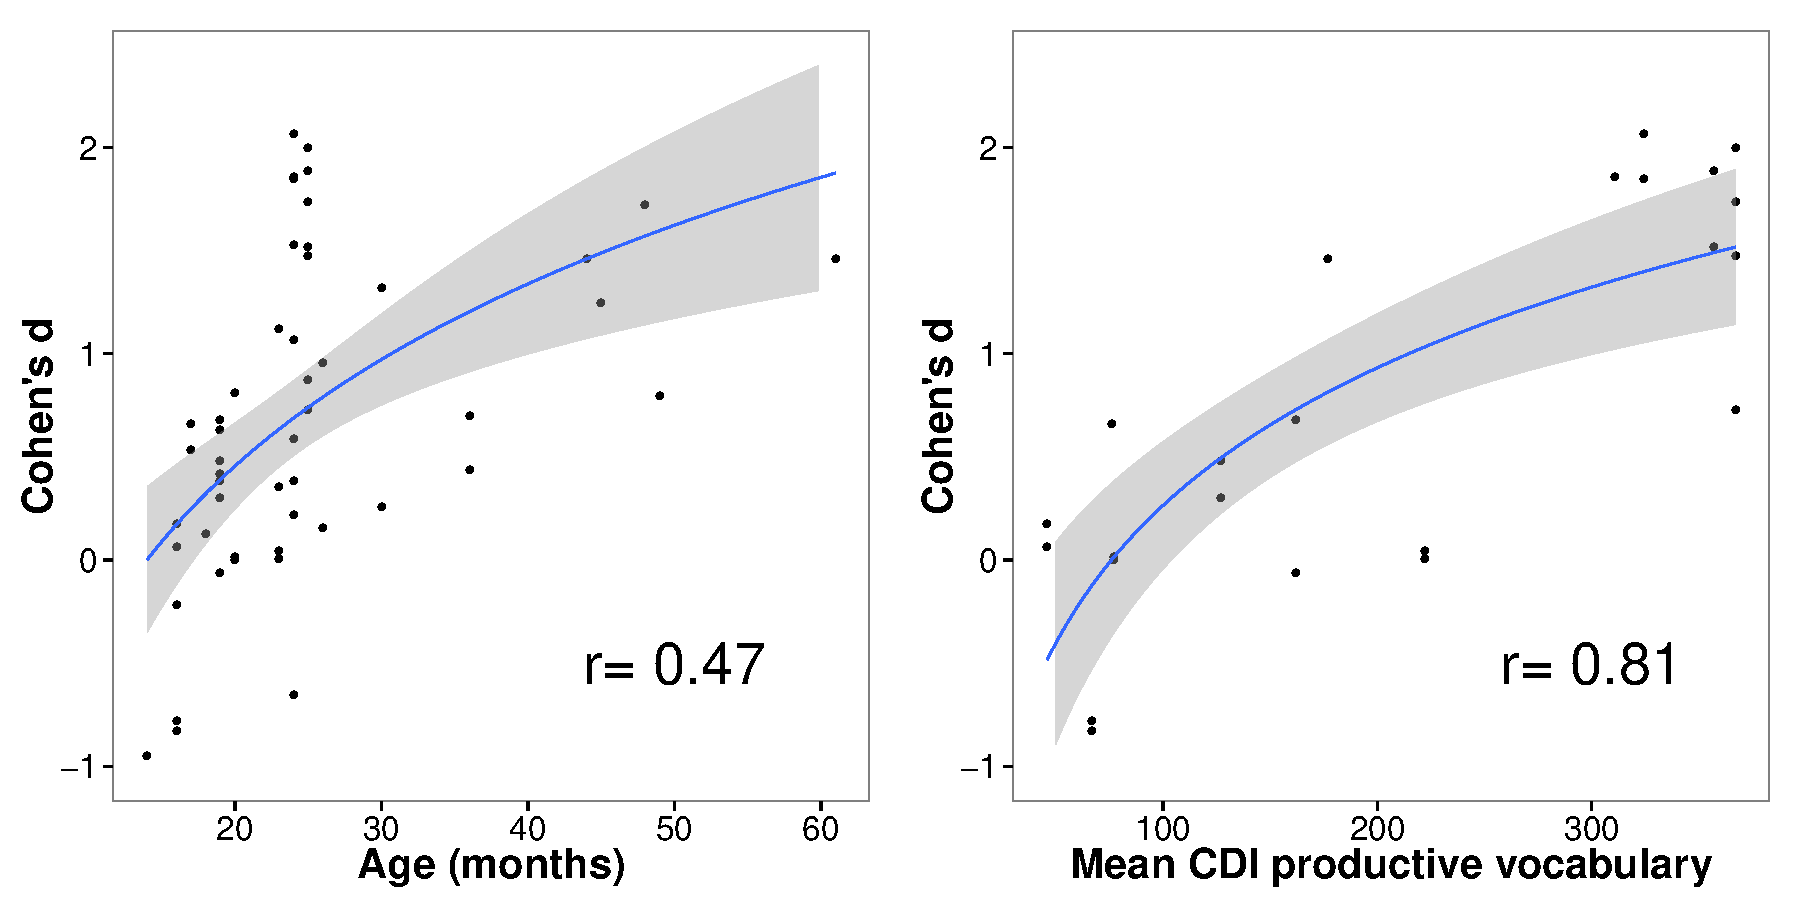
\includegraphics[scale = .5]{figs/d_age_vocab.pdf}
\end{center}
\caption{Effect size in the disambiguation task as a function of age (left) and vocabulary (right), with log fit. Both age and vocabulary are highly correlated with the disambiguation bias. }
\end{figure}


\end{document}


